\section{Results}
\label{sec:results}
% claim: R01
\subsection{Coverage and normal-development correspondence}
Every method produced 897,119 finite eligible final scores: 214,473 in the protected normal slice and 682,646 in the mixed slice. Eligible coverage is 100\%. Raw final coverage is 99.829967\%; the only 1,528 exclusions are the common initial warmup. No missing scores explain the weak detection. Protected-normal exposure is \NormalHours\ hours for every method.

% claim: R02
Earlier normal-only checks supported a recurring 38-second reference and prospective state synchronization, but did not establish accurate latent phase. The synchronized observer's development one-step MSE was \ObserverMSE, compared with \ARMSE\ for the ordinary autoregression. The declared ambiguity criterion was met at \AmbiguityPct\% of sampled diagnostic endpoints. The criterion used normalized entropy above 0.5 or circular resultant below 0.5; these are descriptive diagnostics, not calibrated confidence bounds or independently observed phase errors. This evidence already limited the observer interpretation before final scoring.

% claim: R03
\subsection{Point detection and normal alarm burden}
Table~\ref{tab:results} shows all declared methods in their frozen order. \method{O-RC} achieved F1 \RCFone\ and point recall \RCRecallPct\%. Its protected-normal point alarm fraction was \RCNormalPct\%, with \RCEpisodes\ episodes or \RCEpisodeRate\ episodes per eligible hour. Thus a point-alarm fraction close to the calibration percentile coexisted with frequent alarm episodes. No method exceeded \TemplateRecallPct\% point recall.

\begin{table}[htbp]\centering\scriptsize
\caption{Complete final comparison. Precision, recall, F1 and AP are fractions. Normal point alarms are percentages; episodes/h uses eligible protected-normal exposure. Hits are event overlaps out of eight. No scores are point-adjusted.}\label{tab:results}
\resizebox{\textwidth}{!}{\begin{tabular}{lrrrrrrr}
\toprule
Method & Precision & Recall & F1 & AP & Normal (\%) & Episodes/h & Hits \\
\midrule
O-R & 0.465869 & 0.008452 & 0.016603 & 0.506108 & 1.0067 & 189.34 & 7/8 \\
O-RC & 0.478459 & 0.008805 & 0.017292 & 0.506414 & 0.9941 & 185.98 & 8/8 \\
O-C & 0.509185 & 0.009705 & 0.019047 & 0.506135 & 0.9861 & 342.76 & 8/8 \\
O-K & 0.505838 & 0.009777 & 0.019183 & 0.506193 & 0.9917 & 349.47 & 8/8 \\
O-L & 0.465875 & 0.008513 & 0.016720 & 0.506284 & 1.0053 & 189.34 & 7/8 \\
O-Rv & 0.465476 & 0.008446 & 0.016591 & 0.502845 & 1.0048 & 189.34 & 7/8 \\
O-Follow & 0.465551 & 0.008368 & 0.016441 & 0.504844 & 1.0043 & 189.34 & 7/8 \\
O-Free & 0.466422 & 0.008461 & 0.016620 & 0.506295 & 0.9964 & 189.34 & 7/8 \\
V-Z & 0.462248 & 0.008414 & 0.016528 & 0.506759 & 0.9969 & 189.34 & 7/8 \\
T-32 & 0.527677 & 0.040217 & 0.074737 & 0.490596 & 1.3997 & 200.42 & 8/8 \\
AR-4 & 0.500603 & 0.009604 & 0.018846 & 0.507711 & 0.9833 & 437.09 & 8/8 \\
\bottomrule
\end{tabular}
}
\end{table}

\begin{figure}[htbp]\centering
\begin{tikzpicture}
\begin{groupplot}[group style={group size=3 by 1,horizontal sep=0.65cm},width=0.29\textwidth,height=8cm,xbar,/pgf/bar width=5pt,ymin=-0.7,ymax=10.7,ytick={0,...,10},yticklabels={O-R,O-RC,O-C,O-K,O-L,O-Rv,O-Follow,O-Free,V-Z,T-32,AR-4},y dir=reverse,xmin=0,tick label style={font=\scriptsize},label style={font=\small},xmajorgrids=true,grid style={gray!20}]
\nextgroupplot[xlabel={Point recall (\%)}]
\addplot[fill=blue!55,draw=blue!80!black] coordinates {(0.8451918681,0) (0.8804925897,1) (0.9704804949,2) (0.9777142493,3) (0.8512682218,4) (0.8446131677,5) (0.836800713,6) (0.8460599186,7) (0.8414303158,8) (4.021678115,9) (0.9603532387,10)};
\nextgroupplot[xlabel={Normal alarms (\%)},yticklabels={}]
\addplot[fill=blue!55,draw=blue!80!black] coordinates {(1.006653518,0) (0.9940645209,1) (0.9861381153,2) (0.9917332252,3) (1.005254741,4) (1.004788482,5) (1.004322222,6) (0.9963958167,7) (0.9968620759,8) (1.399709987,9) (0.9833405604,10)};
\nextgroupplot[xlabel={Normal episodes/h},yticklabels={}]
\addplot[fill=blue!55,draw=blue!80!black] coordinates {(189.3394009,0) (185.9823194,1) (342.758029,2) (349.4721922,3) (189.3394009,4) (189.3394009,5) (189.3394009,6) (189.3394009,7) (189.3394009,8) (200.4177702,9) (437.0920213,10)};
\end{groupplot}
\end{tikzpicture}

\caption{Detection and false-alarm burden for every declared method. Axes use different units as labelled; bars start at zero. This descriptive figure has no independent-acquisition uncertainty intervals. Values are generated from the saved final summary.}\label{fig:tradeoffs}
\end{figure}

% claim: R04
The primary \method{O-RC} minus \method{O-R} contrast increased F1 by \FoneGain. It added 122 true-positive points while removing 32 mixed false-positive points, 27 protected-normal alarm points and ten protected-normal episodes. Normal episode rate decreased by 3.3571/hour. These paired recorded outcomes are slightly favorable to the added correction term, with unchanged coverage. Their small size and low absolute recall do not establish useful general detection or a newly effective security mechanism.

% claim: R05
The ordinary \method{AR-4} achieved F1 \ARFone\ and AP \ARAP, both above \method{O-RC}, with slightly fewer normal alarm points (2,109 versus 2,132). It produced 1,302 normal episodes, or \AREpisodeRate/hour, compared with 554 for \method{O-RC}. The fixed template \method{T-32} achieved the largest F1 (\TemplateFone) and recall (\TemplateRecallPct\%), but its normal point alarms reached \TemplateNormalPct\% and mixed scheduled-zero alarms 3.6912\%. These are trade-offs, not a single global ranking. No scalar utility was declared to choose a winner after exposure.

% claim: R06
Mixed positive prevalence was \PrevalencePct\%. The constant tied-score AP reference is that prevalence; observed AP ranged from 0.490596 to 0.507711. Values near this reference do not establish useful broad ranking separation. This reference is arithmetic, not an additional detector run. Precision reflects the recorded schedule's unusually high positive prevalence and is not an estimated field attack precision.

% claim: R07
\subsection{Explanatory scores and update-policy ablations}
Correction-only \method{O-C} and KL surprise \method{O-K} had slightly higher F1 than \method{O-RC}, but 342.76 and 349.47 normal episodes/hour, respectively. The energy score \method{O-L}, velocity residual \method{O-Rv}, free-running and unconstrained-following residuals remained close to \method{O-R} on the reported point outcomes. The direct velocity control was also similar. These are descriptive similarities, not evidence from an equivalence test. They do not isolate a causal benefit of progression, nor justify attributing detection to a uniquely observer-specific mechanism. The free-running variant's diffusive near-uniform state is a limitation of that particular ablation.

% claim: R08
\subsection{All eight events and schedule-relative delay}
No method had an alarm already active at any of the eight event starts. In this recording, every overlap hit therefore also had a fresh onset. \method{O-R}, \method{O-L}, \method{O-Rv}, \method{O-Follow}, \method{O-Free} and \method{V-Z} missed event 5 entirely. Each remaining method hit all eight. Appendix~\ref{app:events} retains every delay and miss, and every scheduled-zero recovery interval.

\begin{figure}[htbp]\centering
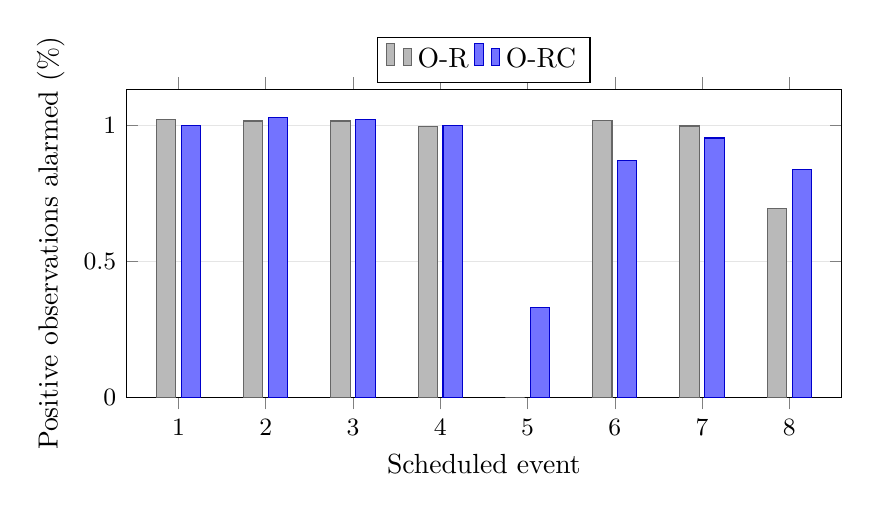
\begin{tikzpicture}
\begin{axis}[width=0.88\textwidth,height=5.5cm,ybar,bar width=7pt,xmin=0.4,xmax=8.6,ymin=0,xtick={1,...,8},xlabel={Scheduled event},ylabel={Positive observations alarmed (\%)},legend style={at={(0.5,1.02)},anchor=south,legend columns=2},ymajorgrids=true,grid style={gray!20},tick label style={font=\small}]
\addplot[fill=gray!55,draw=gray!80!black] coordinates {(1,1.023124465) (2,1.016203704) (3,1.016203704) (4,0.9953703704) (5,0) (6,1.018518519) (7,0.9976851852) (8,0.6944283697)};
\addplot[fill=blue!55,draw=blue!80!black] coordinates {(1,0.9999768524) (2,1.030092593) (3,1.020833333) (4,1) (5,0.3310185185) (6,0.8703703704) (7,0.9537037037) (8,0.8379435661)};
\legend{O-R,O-RC}
\end{axis}
\end{tikzpicture}

\caption{Fraction of positive observations alarmed within each event for the matched primary pair. Event 5 has no \method{O-R} alarm. Eight \method{O-RC} event hits coexist with sparse point coverage inside the long intervals.}\label{fig:eventcoverage}
\end{figure}

% claim: R09
\method{O-RC} first alarmed 9.20 seconds after the event-5 schedule flag. On the seven events both primary methods hit, five first-alarm delays were identical; \method{O-RC} was 2.05 seconds later on event 6 and approximately 0.05 seconds later on event 7. It was not earlier on any shared hit. Its detected-only median of 9.45 seconds, compared with 9.70 seconds for \method{O-R}, uses eight and seven events respectively and cannot establish faster matched detection.

% claim: R10
Each scheduled interval contains more than 43,000 positive observations. Any one alarm suffices for an overlap hit. \method{O-RC}'s eight hits therefore coexist with 342,559 false-negative positive observations, frequent normal episodes and AP near the prevalence reference. Short first-alarm delays here do not imply sustained recognition of the scheduled deviation or verified detection of its physical onset.

% claim: R11
\subsection{Measured resources}
Table~\ref{tab:resources} reports the whole-worker measurements. Both phases stayed within their frozen caps: scoring 900 seconds wall/600 seconds CPU and evaluation 1,800/1,200 seconds; both allowed 1 GiB worker resident memory and 256 MiB output. The hardware was a local Apple M5 Pro with 24 GiB host memory, using Python 3.15.0 and the standard library. No GPU or paid compute was used.

\begin{table}[htbp]\centering\small
\caption{Whole-phase resources, including source checks, parsing and output work. These are not isolated inference measurements.}\label{tab:resources}
\resizebox{\textwidth}{!}{\begin{tabular}{lrrrr}
\toprule
Phase & Wall (s) & CPU (s) & Peak RSS (MiB) & Output (MiB) \\
\midrule
score-final & 270.890 & 270.520 & 143.19 & 102.317 \\
evaluate-final & 44.778 & 44.660 & 902.50 & 0.188 \\
\bottomrule
\end{tabular}
}
\end{table}

% claim: R12
Per-method processing costs, initialization/parsing decomposition and per-record latency quantiles were not instrumented. The recorded whole-roster execution is locally feasible under its limits, but cannot determine whether the correction term's small gain had a measurable compute advantage or penalty relative to a control. No edge-device, transport-latency or live-deployment conclusion follows.
